
% Configuración específica para anexos (contador completamente independiente)
\newcounter{anexo} % Crear un contador específico para anexos
\setcounter{anexo}{0} % Inicializar en 0
\renewcommand{\theanexo}{\Alph{anexo}} % Formato alfabético para anexos

% Redefinir el formato del capítulo para que muestre "Anexo" correctamente
\titleformat{\chapter}[display]
{\normalfont\huge\bfseries}{Anexo\ \theanexo}{20pt}{\Huge}

% Aplicar estilo de página para anexos
\pagestyle{anexos}

%--------------------------------------------------------------------------------
\FloatBarrier
\cleardoublepage
\refstepcounter{anexo} % Incrementar el contador de anexo
\phantomsection
\addcontentsline{toc}{chapter}{Anexo \theanexo: Elementos en ArchiMate}

% Mostrar manualmente el título del anexo sin línea
\vspace{40pt}
{\centering \normalfont\huge\bfseries Anexo \theanexo: Elementos en ArchiMate \par}
\vspace{40pt}

\label{anexo:archimate-elementos}
\markboth{Anexo \theanexo: Elementos en ArchiMate}{Anexo \theanexo: Elementos en ArchiMate}
\noindent
Este anexo presenta una descripción detallada de los elementos y relaciones del lenguaje de modelado ArchiMate, proporcionando una referencia completa para la comprensión y aplicación de este estándar en arquitectura empresarial.

\noindent
\noindent
La presente sección del anexo se fundamenta en el trabajo de grado desarrollado por Michael Stiven Honores Quishpillo y Juan David Naranjo Sánchez, titulado ``Propuesta de Transformación Digital para la Gestión de la Información en el Proceso de Producción Establecido en la Organización Prefabricados JAMAR Validada a través de la Construcción de un Prototipo Funcional''.

\section{Elementos de negocio}

\begin{longtable}{|c|p{8cm}|}
	\caption{Elementos de negocio en ArchiMate} \label{tab:elementos-negocio-archimate}                                                  \\
	\hline
	\textbf{Icono}                                             & \textbf{Descripción}                                                    \\
	\hline
	\endfirsthead

	\caption[]{Elementos de negocio en ArchiMate (continuación)}                                                                         \\
	\hline
	\textbf{Icono}                                             & \textbf{Descripción}                                                    \\
	\hline
	\endhead

	\hline
	\endfoot

	\endlastfoot
	\includegraphics{anexos/ARCHI/business/actor.png}          &
	\textbf{Business Actor:} Corresponde a una entidad capaz de ejecutar comportamientos dentro del contexto organizacional, como puede ser una persona o una organización. \\
	\hline
	\includegraphics{anexos/ARCHI/business/rol.png}            &
	\textbf{Business Role:} Representa el conjunto de responsabilidades y comportamientos que pueden ser asumidos por un actor dentro del negocio. \\
	\hline
	\includegraphics{anexos/ARCHI/business/colaboration.png}   &
	\textbf{Business Collaboration:} Se refiere a la agrupación de dos o más roles de negocio que cooperan para alcanzar un objetivo común. \\
	\hline
	\includegraphics{anexos/ARCHI/business/interface.png}      &
	\textbf{Business Interface:} Constituye un punto de acceso mediante el cual un servicio de negocio es ofrecido a los actores. \\
	\hline
	\includegraphics{anexos/ARCHI/business/process.png}        &
	\textbf{Business Process:} Conjunto estructurado de actividades orientadas a la obtención de un resultado específico para un cliente interno o externo. \\
	\hline
	\includegraphics{anexos/ARCHI/business/function.png}       &
	\textbf{Business Function:} Agrupación de comportamientos que comparten una misma base de recursos dentro del negocio. \\
	\hline
	\includegraphics{anexos/ARCHI/business/interaction.png}    &
	\textbf{Business Interaction:} Describe un comportamiento que surge de la interacción entre dos o más roles de negocio. \\
	\hline
	\includegraphics{anexos/ARCHI/business/service.png}        &
	\textbf{Business Service:} Representa un servicio que satisface una necesidad de un cliente, ya sea interno o externo a la organización. \\
	\hline
	\includegraphics{anexos/ARCHI/business/event.png}          &
	\textbf{Business Event:} Hace referencia a un suceso que impacta la continuidad o el flujo de un proceso de negocio. \\
	\hline
	\includegraphics{anexos/ARCHI/business/object.png}         &
	\textbf{Business Object:} Concepto utilizado dentro de un dominio específico del negocio. \\
	\hline
	\includegraphics{anexos/ARCHI/business/contract.png}       &
	\textbf{Contract:} Acuerdo, ya sea formal o informal, que define los derechos y obligaciones asociados a un producto. \\
	\hline
	\includegraphics{anexos/ARCHI/business/representation.png} &
	\textbf{Representation:} Forma en la que la información contenida en un objeto de negocio se presenta o es percibida. \\
	\hline
	\includegraphics{anexos/ARCHI/business/product.png}        &
	\textbf{Product:} Conjunto coherente de servicios y/o objetos pasivos, acompañado de acuerdos o contratos que lo respaldan. \\
	\hline
	\includegraphics{anexos/ARCHI/business/grouping.png}       &
	\textbf{Grouping:} Mecanismo utilizado para organizar y agrupar elementos relacionados dentro de un modelo de arquitectura. \\                                  \\
\end{longtable}

\section{Elementos de aplicación}

\begin{longtable}{|c|p{8cm}|}
	\caption{Elementos de aplicación en ArchiMate} \label{tab:elementos-aplicacion-archimate}                                                            \\
	\hline
	\textbf{Icono}                                               & \textbf{Descripción}                                                                  \\
	\hline
	\endfirsthead

	\caption[]{Elementos de aplicación en ArchiMate (continuación)}                                                                                      \\
	\hline
	\textbf{Icono}                                               & \textbf{Descripción}                                                                  \\
	\hline
	\endhead

	\hline
	\endfoot

	\endlastfoot
	\includegraphics{anexos/ARCHI/application/component.png}     &
	\textbf{Application Component:} Unidad modular que proporciona un conjunto de servicios relacionados dentro del ámbito de las aplicaciones. \\
	\hline
	\includegraphics{anexos/ARCHI/application/collaboration.png} &
	\textbf{Application Collaboration:} Interacción establecida entre dos o más componentes de aplicación que cooperan entre sí. \\
	\hline
	\includegraphics{anexos/ARCHI/application/interface.png}     &
	\textbf{Application Interface:} Punto de acceso a las funcionalidades que ofrece una aplicación. \\
	\hline
	\includegraphics{anexos/ARCHI/application/process.png}       &
	\textbf{Application Process:} Conjunto de comportamientos ejecutados por uno o varios componentes de aplicación con el fin de alcanzar un objetivo determinado. \\
	\hline
	\includegraphics{anexos/ARCHI/application/function.png}      &
	\textbf{Application Function:} Agrupación de comportamientos relacionados en el contexto de las aplicaciones. \\
	\hline
	\includegraphics{anexos/ARCHI/application/interaction.png}   &
	\textbf{Application Interaction:} Describe el comportamiento resultante de la interacción entre dos o más componentes de aplicación. \\
	\hline
	\includegraphics{anexos/ARCHI/application/service.png}       &
	\textbf{Application Service:} Servicio que una aplicación expone hacia su entorno. \\
	\hline
	\includegraphics{anexos/ARCHI/application/event.png}         &
	\textbf{Application Event:} Evento que ocurre y afecta la continuidad de un proceso dentro del contexto de aplicaciones. \\
	\hline
	\includegraphics{anexos/ARCHI/application/object.png}        &
	\textbf{Data Object:} Objeto pasivo que es manipulado por comportamientos dentro del entorno de aplicaciones.                       \\
	\hline
\end{longtable}

\section{Elementos tecnológicos}

\begin{longtable}{|c|p{8cm}|}
	\caption{Elementos tecnológicos en ArchiMate} \label{tab:elementos-tecnologicos-archimate}                                                    \\
	\hline
	\textbf{Icono}                                              & \textbf{Descripción}                                                            \\
	\hline
	\endfirsthead

	\caption[]{Elementos tecnológicos en ArchiMate (continuación)}                                                                                \\
	\hline
	\textbf{Icono}                                              & \textbf{Descripción}                                                            \\
	\hline
	\endhead

	\hline
	\endfoot

	\endlastfoot
	\includegraphics{anexos/ARCHI/technology/facility.png}      &
	\textbf{Facility:} Espacio físico o infraestructura destinada al alojamiento de recursos tecnológicos. \\
	\hline
	\includegraphics{anexos/ARCHI/technology/equipment.png}     &
	\textbf{Equipment:} Recurso físico que puede ser utilizado en la ejecución de procesos organizacionales. \\
	\hline
	\includegraphics{anexos/ARCHI/technology/material.png}      &
	\textbf{Material:} Recursos físicos o insumos empleados o generados en el desarrollo de procesos empresariales. \\
	\hline
	\includegraphics{anexos/ARCHI/technology/node.png}          &
	\textbf{Node:} Recurso computacional encargado de alojar, procesar o interactuar con otros recursos y aplicaciones. \\
	\hline
	\includegraphics{anexos/ARCHI/technology/device.png}        &
	\textbf{Device:} Recurso físico capaz de ejecutar software de sistema o componentes de aplicación. \\
	\hline
	\includegraphics{anexos/ARCHI/technology/software.png}      &
	\textbf{System Software:} Software que proporciona la base necesaria para la ejecución de aplicaciones, como sistemas operativos o middleware. \\
	\hline
	\includegraphics{anexos/ARCHI/technology/collaboration.png} &
	\textbf{Technology Collaboration:} Interacción entre dos o más nodos o dispositivos que trabajan de manera conjunta. \\
	\hline
	\includegraphics{anexos/ARCHI/technology/interface.png}     &
	\textbf{Technology Interface:} Punto de acceso a través del cual un nodo o dispositivo ofrece sus funcionalidades. \\
	\hline
	\includegraphics{anexos/ARCHI/technology/process.png}       &
	\textbf{Technology Process:} Conjunto de comportamientos tecnológicos orientados al logro de un objetivo específico. \\
	\hline
	\includegraphics{anexos/ARCHI/technology/function.png}      &
	\textbf{Technology Function:} Agrupación de comportamientos tecnológicos relacionados entre sí. \\
	\hline
	\includegraphics{anexos/ARCHI/technology/interaction.png}   &
	\textbf{Technology Interaction:} Describe la interacción entre dos o más nodos o dispositivos. \\
	\hline
	\includegraphics{anexos/ARCHI/technology/service.png}       &
	\textbf{Technology Service:} Servicio proporcionado por la capa tecnológica a su entorno. \\
	\hline
	\includegraphics{anexos/ARCHI/technology/event.png}         &
	\textbf{Technology Event:} Evento que ocurre y afecta la continuidad de un proceso tecnológico. \\
	\hline
	\includegraphics{anexos/ARCHI/technology/artifact.png}      &
	\textbf{Artifact:} Objeto físico de información utilizado o generado en procesos tecnológicos. \\
	\hline
	\includegraphics{anexos/ARCHI/technology/network.png}       &
	\textbf{Communication Network:} Infraestructura que posibilita la comunicación entre nodos y dispositivos. \\
	\hline
	\includegraphics{anexos/ARCHI/technology/path.png}          &
	\textbf{Path:} Conexión que define el flujo de datos entre nodos o dispositivos. \\
	\hline
	\includegraphics{anexos/ARCHI/technology/distribution.png}  &
	\textbf{Distribution Network:} Red que facilita la distribución de productos o recursos a través de una infraestructura.                   \\
	\hline
\end{longtable}


\noindent
Si bien el lenguaje ArchiMate contempla capas adicionales como estrategia y relaciones, en el presente trabajo no se consideraron dichas capas, dado que el alcance del modelo se centra en la representación de los niveles de negocio, aplicación y tecnología.

%--------------------------------------------------------------------------------
\FloatBarrier
\cleardoublepage
\refstepcounter{anexo}
\phantomsection
\addcontentsline{toc}{chapter}{Anexo \theanexo: Resultados individuales de la encuesta de percepción}

\vspace{40pt}
{\centering \normalfont\huge\bfseries Anexo \theanexo: Resultados individuales de la encuesta de percepción \par}
\vspace{40pt}

\label{anx:resultados_encuesta}
\markboth{Anexo \theanexo: Resultados individuales de la encuesta de percepción}{Anexo \theanexo: Resultados individuales de la encuesta de percepción}
\noindent
Las siguientes tablas presentan la distribución de frecuencias de respuestas por ítem para cada sección de la encuesta de percepción aplicada al grupo experimental. Dado que la encuesta fue respondida de forma anónima, los resultados se presentan agregados por valor de escala, indicando cuántos de los cuatro subgrupos respondientes seleccionaron cada opción. Los valores corresponden a una escala Likert de 1 a 5, donde 1 representa total desacuerdo y 5 total acuerdo.

\begin{table}[H]
\centering
\caption{Distribución de frecuencias por ítem -- Sección 1: Comprensión de la notación}
\label{tab:frecuencias_seccion1}
\begin{tabular}{|p{7cm}|c|c|c|c|c|c|}
\hline
\textbf{Ítem} & \textbf{1} & \textbf{2} & \textbf{3} & \textbf{4} & \textbf{5} & \textbf{Prom.} \\
\hline
Los elementos de la notación fueron fáciles de entender. & 0 & 0 & 0 & 4 & 0 & 4.00 \\
\hline
La organización por capas facilitó la comprensión del modelo. & 0 & 0 & 0 & 1 & 3 & 4.75 \\
\hline
Los ejemplos proporcionados ayudaron a entender cómo usar la notación. & 0 & 0 & 0 & 0 & 4 & 5.00 \\
\hline
Los nombres y descripciones de los elementos fueron claros. & 0 & 0 & 0 & 2 & 2 & 4.50 \\
\hline
\end{tabular}
\end{table}

\begin{table}[H]
\centering
\caption{Distribución de frecuencias por ítem -- Sección 2: Uso de los elementos}
\label{tab:frecuencias_seccion2}
\begin{tabular}{|p{7cm}|c|c|c|c|c|c|}
\hline
\textbf{Ítem} & \textbf{1} & \textbf{2} & \textbf{3} & \textbf{4} & \textbf{5} & \textbf{Prom.} \\
\hline
Pude identificar fácilmente qué elementos usar para representar el problema. & 0 & 0 & 1 & 2 & 1 & 4.00 \\
\hline
La cantidad de elementos fue adecuada (ni excesiva ni insuficiente). & 0 & 0 & 0 & 3 & 1 & 4.25 \\
\hline
Me sentí cómodo utilizando los elementos durante el ejercicio. & 0 & 0 & 0 & 4 & 0 & 4.00 \\
\hline
\end{tabular}
\end{table}

\begin{table}[H]
\centering
\caption{Distribución de frecuencias por ítem -- Sección 3: Expresividad y utilidad}
\label{tab:frecuencias_seccion3}
\begin{tabular}{|p{7cm}|c|c|c|c|c|c|}
\hline
\textbf{Ítem} & \textbf{1} & \textbf{2} & \textbf{3} & \textbf{4} & \textbf{5} & \textbf{Prom.} \\
\hline
La notación me permitió representar el problema de forma clara. & 0 & 0 & 0 & 2 & 2 & 4.50 \\
\hline
La notación facilita la comprensión del sistema representado. & 0 & 0 & 0 & 2 & 2 & 4.50 \\
\hline
Considero que la notación es útil para modelar sistemas reales. & 0 & 0 & 0 & 1 & 3 & 4.75 \\
\hline
\end{tabular}
\end{table}

\begin{table}[H]
\centering
\caption{Distribución de frecuencias por ítem -- Sección 4: Experiencia general}
\label{tab:frecuencias_seccion4}
\begin{tabular}{|p{7cm}|c|c|c|c|c|c|}
\hline
\textbf{Ítem} & \textbf{1} & \textbf{2} & \textbf{3} & \textbf{4} & \textbf{5} & \textbf{Prom.} \\
\hline
La notación fue fácil de aprender. & 0 & 0 & 2 & 2 & 0 & 3.50 \\
\hline
Me gustaría utilizar esta notación en otros contextos académicos. & 0 & 0 & 1 & 2 & 1 & 4.00 \\
\hline
Considero que la notación es adecuada para estudiantes en formación. & 0 & 0 & 1 & 1 & 2 & 4.25 \\
\hline
\end{tabular}
\end{table}
\noindent
\textit{Nota: Los valores 1 y 2 no fueron seleccionados en ningún ítem. 
La escala completa se presenta para mantener la integridad del instrumento.}

--------------------------------------------------------------------------------
\FloatBarrier
\cleardoublepage
\refstepcounter{anexo}
\phantomsection
\addcontentsline{toc}{chapter}{Anexo \theanexo: Respuestas abiertas de la encuesta de percepción}

\vspace{40pt}
{\centering \normalfont\huge\bfseries Anexo \theanexo: Respuestas abiertas de la encuesta de percepción \par}
\vspace{40pt}

\label{anx:respuestas_abiertas}
\markboth{Anexo \theanexo: Respuestas abiertas de la encuesta de percepción}{Anexo \theanexo: Respuestas abiertas de la encuesta de percepción}
\noindent
Las siguientes tablas presentan las respuestas abiertas recopiladas en la encuesta de percepción aplicada al grupo experimental, transcritas de forma fiel y sin modificaciones con el fin de preservar la integridad de los datos originales. Dado que la encuesta fue respondida de forma anónima, cada respuesta se identifica únicamente mediante un código de participante (P1, P2, P3).

\begin{table}[H]
\centering
\caption{Respuestas abiertas -- Pregunta 1:  \textquestiondown~Qué fue lo más fácil de entender de la notación?}
\label{tab:abiertas_p1}
\begin{tabular}{|c|p{11cm}|}
\hline
\textbf{Participante} & \textbf{Respuesta} \\
\hline
P1 & Su clasificación por capas, a mi parecer esto facilita demasiado la comprensión de estas, y ya para aprenderlas completamente simplemente se necesita tiempo para más práctica. \\
\hline
P2 & Que con un estándar definido, no habrá divergencia en los conceptos. \\
\hline
P3 & El ordenamiento en capas y sus respectivos elementos. \\
\hline
\end{tabular}
\end{table}

\begin{table}[H]
\centering
\caption{Respuestas abiertas -- Pregunta 2:  \textquestiondown~Qué elementos o aspectos de la notación mejoraría?}
\label{tab:abiertas_p2}
\begin{tabular}{|c|p{11cm}|}
\hline
\textbf{Participante} & \textbf{Respuesta} \\
\hline
P1 & Los logos un poco más grandes, y tal vez más diferenciación en los colores de cada capa, colores que tengan o más contraste, o que definitivamente sean diferentes (no verdes de distinto tono). \\
\hline
P2 & Logos mas intuitivos. \\
\hline
P3 & Algunos elementos muy generales o a veces 2 cosas parecen representar lo mismo. \\
\hline
\end{tabular}
\end{table}

\begin{table}[H]
\centering
\caption{Respuestas abiertas -- Pregunta 3:  \textquestiondown~Hubo algún momento en el que no supo qué elemento o relación utilizar? Explique.}
\label{tab:abiertas_p3}
\begin{tabular}{|c|p{11cm}|}
\hline
\textbf{Participante} & \textbf{Respuesta} \\
\hline
P1 & En algún momento, mientras leía y trataba de entender la guía de usuario. \\
\hline
P2 & Si, por desconocimiento propio. \\
\hline
P3 & No. \\
\hline
\end{tabular}
\end{table}

\begin{table}[H]
\centering
\caption{Respuestas abiertas -- Comentarios adicionales}
\label{tab:abiertas_p4}
\begin{tabular}{|c|p{11cm}|}
\hline
\textbf{Participante} & \textbf{Respuesta} \\
\hline
P1 & Está bien, con ajustes mínimos y una magnificación de su uso, podría llegar a ser el estándar debido a su simplicidad y ayuda general. \\
\hline
P2 & Ta bueno. \\
\hline
P3 & Muy bacano. \\
\hline
\end{tabular}
\end{table}

% %--------------------------------------------------------------------------------
\FloatBarrier
\cleardoublepage
\refstepcounter{anexo}
\phantomsection
\addcontentsline{toc}{chapter}{Anexo \theanexo: Diagramas del grupo experimental (NDITI)}

\vspace{40pt}
{\centering \normalfont\huge\bfseries Anexo \theanexo: Diagramas del grupo experimental (NDITI) \par}
\vspace{40pt}

\label{anx:diagramas_ndti}
\markboth{Anexo \theanexo: Diagramas del grupo experimental (NDITI)}{Anexo \theanexo: Diagramas del grupo experimental (NDITI)}
\noindent
Los siguientes diagramas fueron elaborados por los cinco subgrupos del grupo experimental durante la actividad de diagramación. Cada subgrupo utilizó la NDITI como marco de referencia para representar el problema de modelado planteado. Los diagramas se presentan sin modificaciones respecto a su versión original.

\clearpage
\begin{figure}[H]
\centering
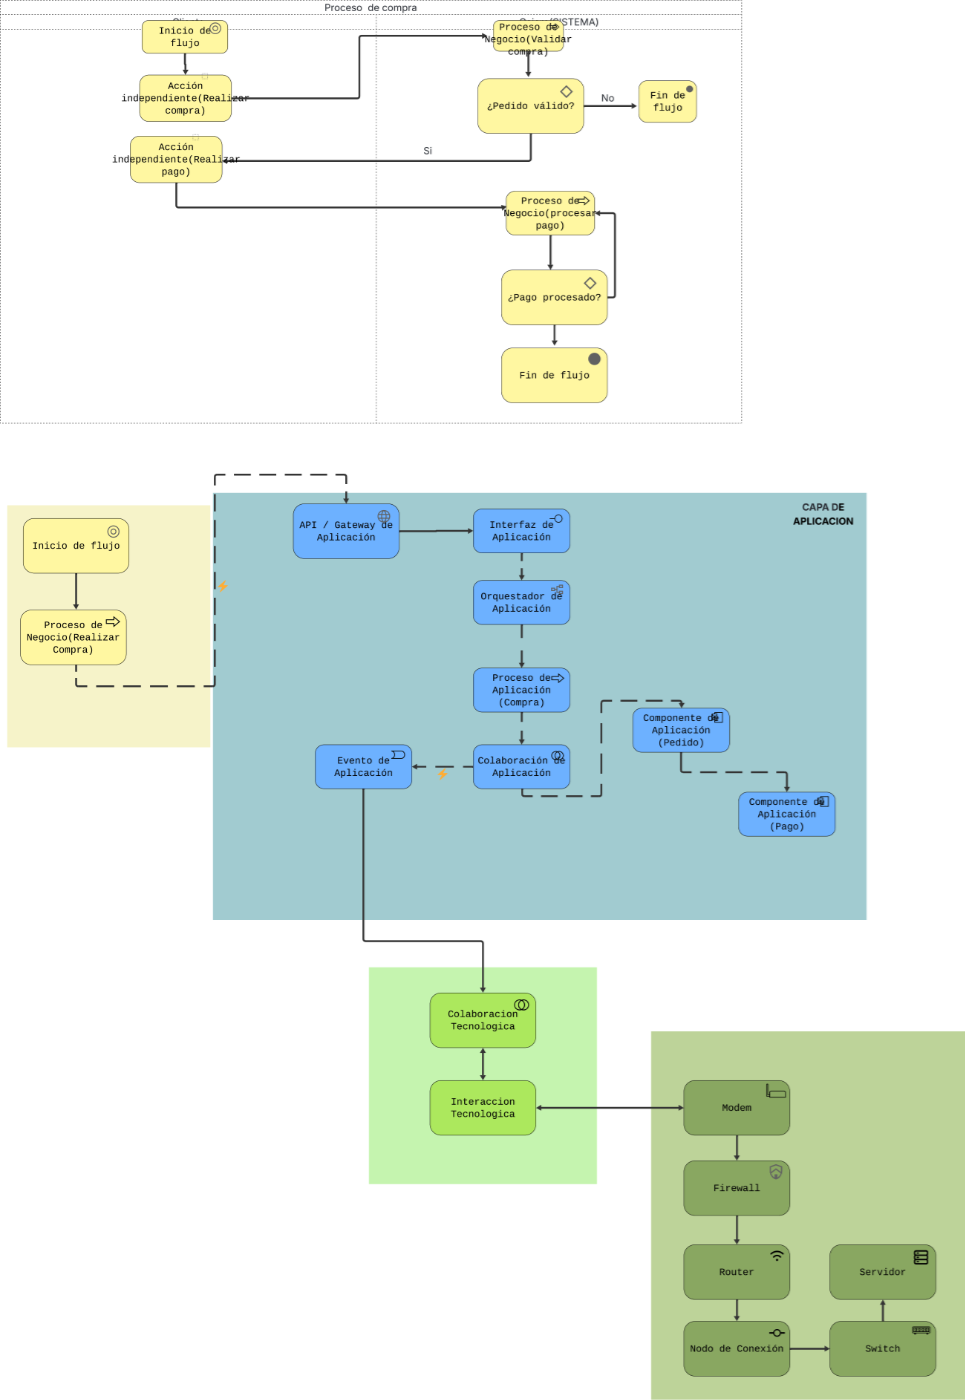
\includegraphics[width=\linewidth,
        height=0.9\textheight,
        keepaspectratio]{tablas-images/diagramas/evaluacion/1S.png}
\caption{Diagrama elaborado por el subgrupo NDITI-1}
\label{fig:diagrama_ndti1}
\end{figure}

\clearpage
\begin{figure}[H]
\centering
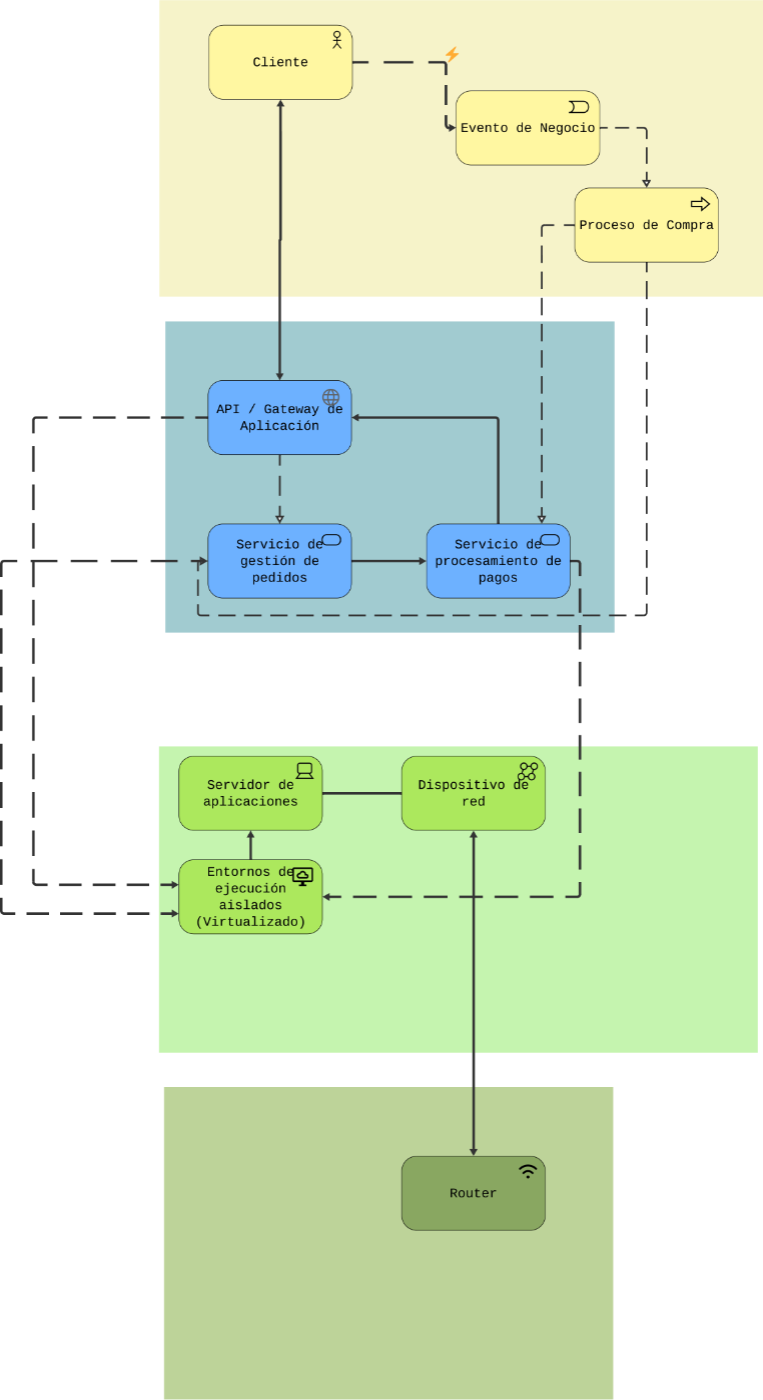
\includegraphics[width=\linewidth,
        height=0.9\textheight,
        keepaspectratio]{tablas-images/diagramas/evaluacion/2S.png}
\caption{Diagrama elaborado por el subgrupo NDITI-2}
\label{fig:diagrama_ndti2}
\end{figure}

\clearpage
\begin{figure}[H]
\centering
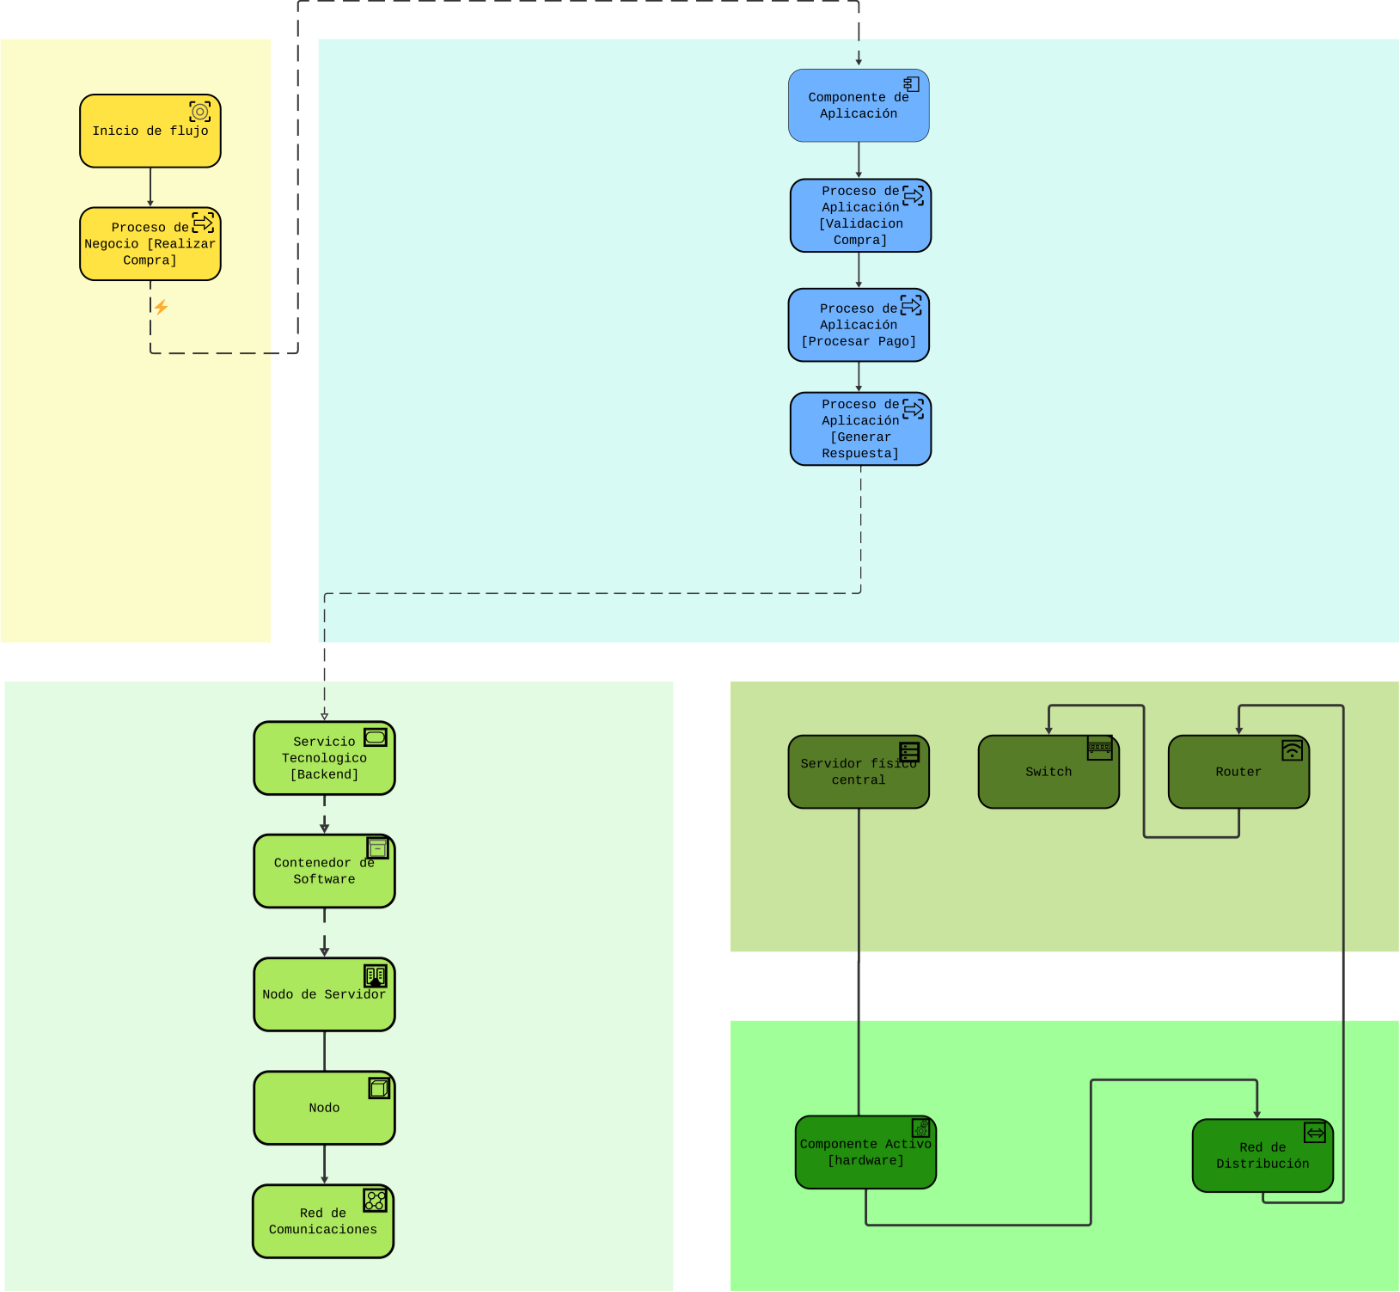
\includegraphics[width=\linewidth,
        height=0.9\textheight,
        keepaspectratio]{tablas-images/diagramas/evaluacion/3S.png}
\caption{Diagrama elaborado por el subgrupo NDITI-3}
\label{fig:diagrama_ndti3}
\end{figure}

\clearpage
\begin{figure}[H]
\centering
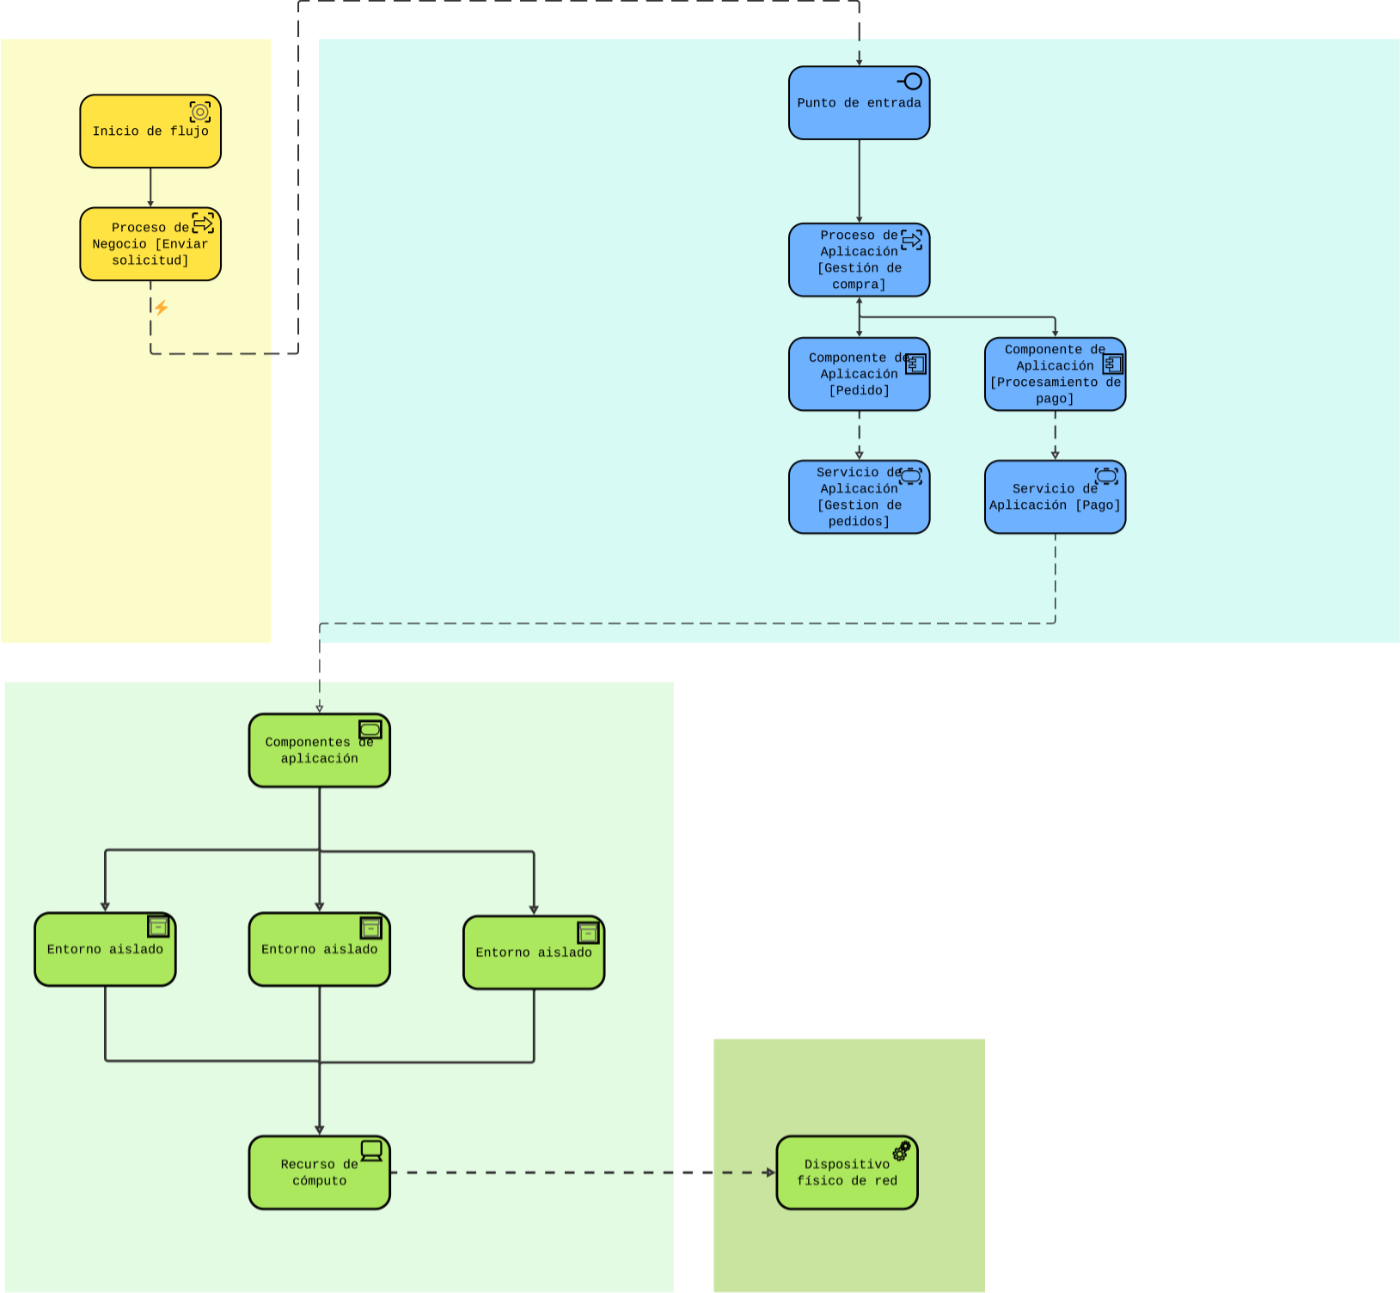
\includegraphics[width=\linewidth,
        height=0.9\textheight,
        keepaspectratio]{tablas-images/diagramas/evaluacion/4S.png}
\caption{Diagrama elaborado por el subgrupo NDITI-4}
\label{fig:diagrama_ndti4}
\end{figure}

\clearpage
\begin{figure}[H]
\centering
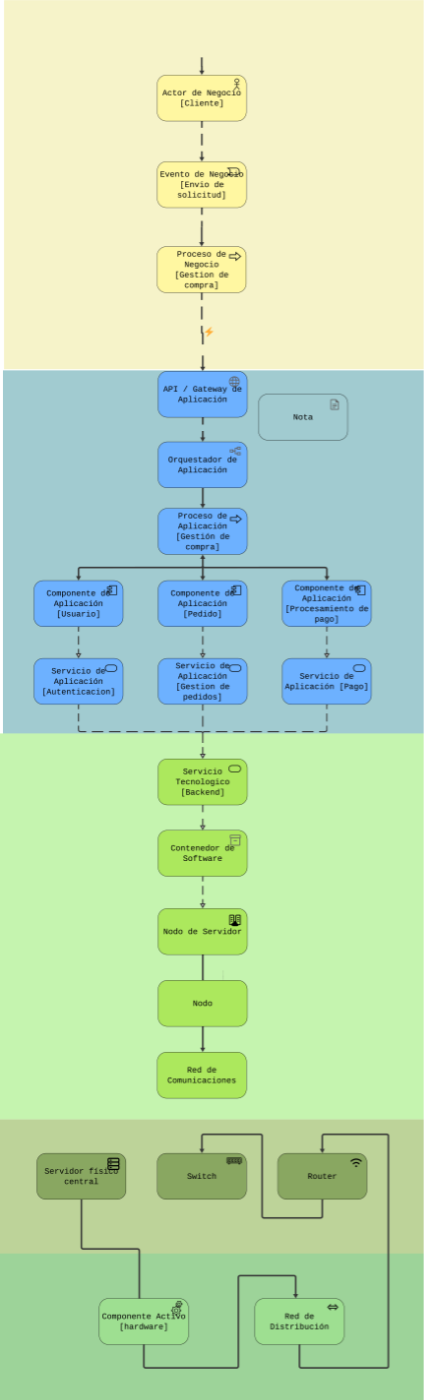
\includegraphics[width=\linewidth,
        height=0.9\textheight,
        keepaspectratio]{tablas-images/diagramas/evaluacion/5S.png}
\caption{Diagrama elaborado por el subgrupo NDITI-5}
\label{fig:diagrama_ndti5}
\end{figure}

 %--------------------------------------------------------------------------------
\FloatBarrier
\cleardoublepage
\refstepcounter{anexo}
\phantomsection
\addcontentsline{toc}{chapter}{Anexo \theanexo: Diagramas del grupo de referencia (libre)}

\vspace{40pt}
{\centering \normalfont\huge\bfseries Anexo \theanexo: Diagramas del grupo de referencia (libre) \par}
\vspace{40pt}

\label{anx:diagramas_libre}
\markboth{Anexo \theanexo: Diagramas del grupo de referencia (libre)}{Anexo \theanexo: Diagramas del grupo de referencia (libre)}
\noindent
Los siguientes diagramas fueron elaborados por los cinco subgrupos del grupo de referencia durante la actividad de diagramación. Cada subgrupo realizó la representación del problema de forma libre, sin un marco de notación definido. Los diagramas se presentan sin modificaciones respecto a su versión original.

\clearpage
\begin{figure}[H]
\centering
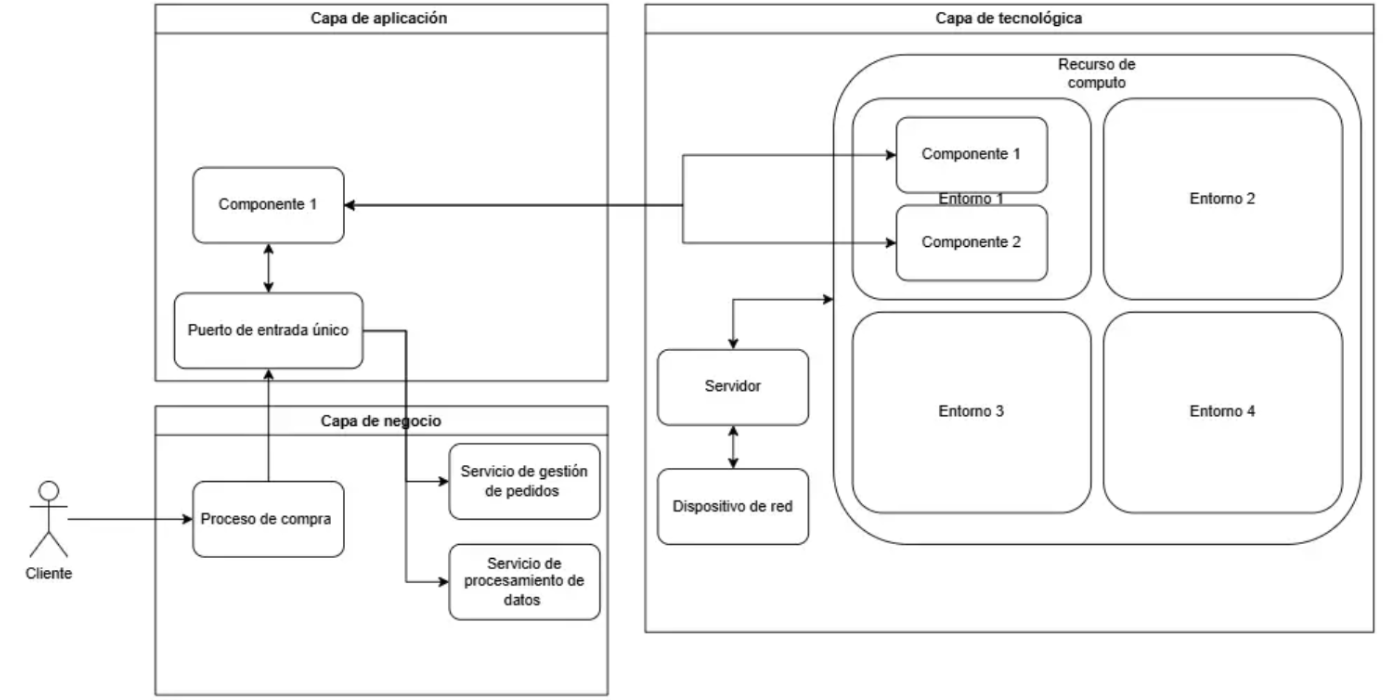
\includegraphics[width=\linewidth,
        height=0.9\textheight,
        keepaspectratio]{tablas-images/diagramas/evaluacion/6S.png}
\caption{Diagrama elaborado por el subgrupo Libre-1}
\label{fig:diagrama_libre1}
\end{figure}

\clearpage
\begin{figure}[H]
\centering
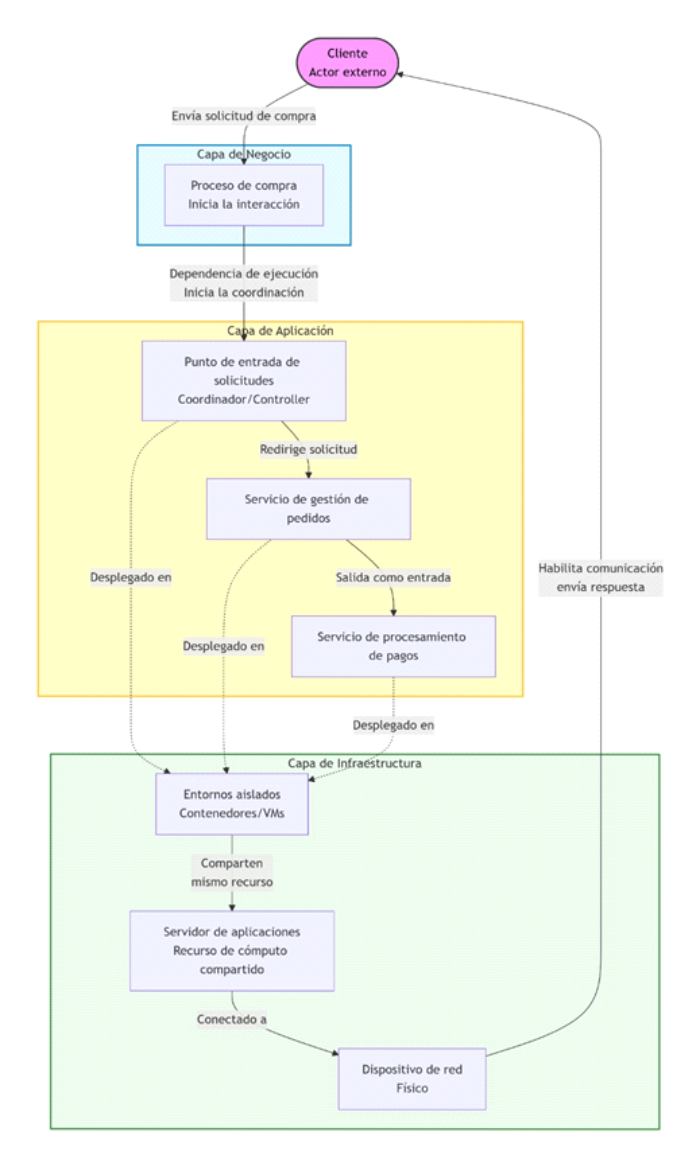
\includegraphics[width=\linewidth,
        height=0.9\textheight,
        keepaspectratio]{tablas-images/diagramas/evaluacion/7S.png}
\caption{Diagrama elaborado por el subgrupo Libre-2}
\label{fig:diagrama_libre2}
\end{figure}

\clearpage
\begin{figure}[H]
\centering
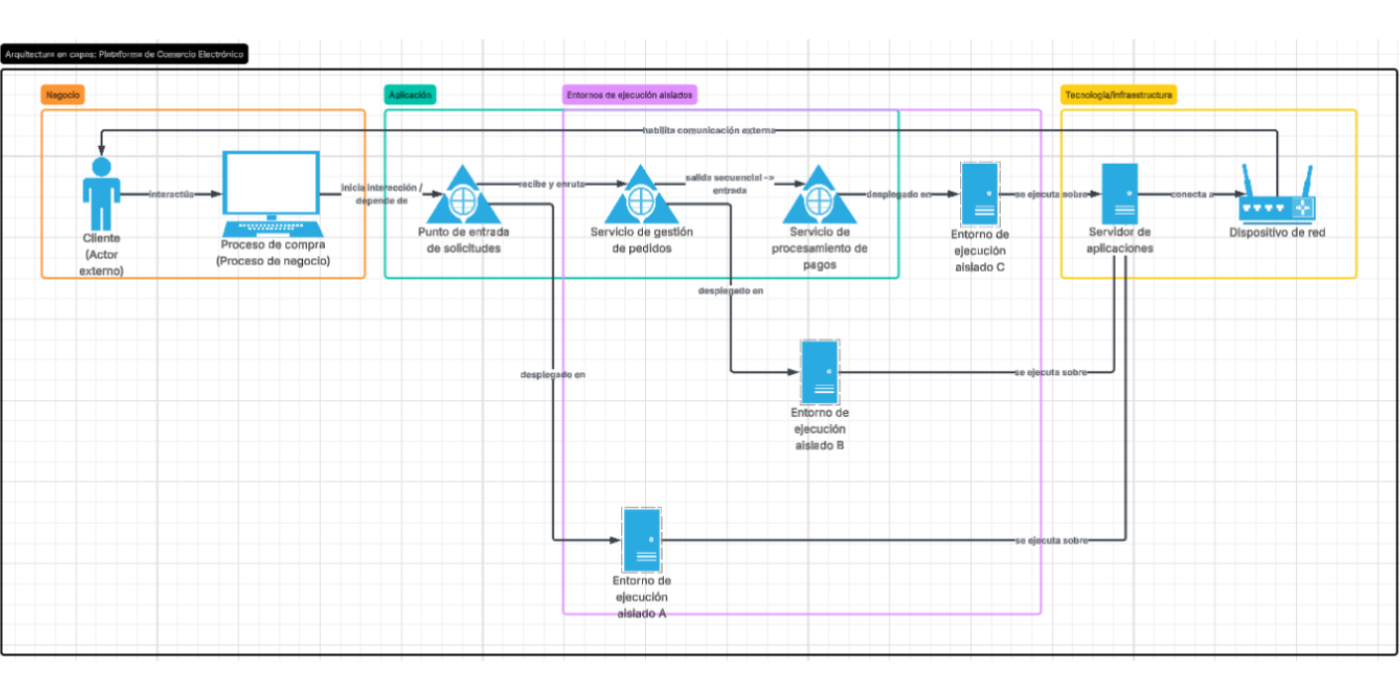
\includegraphics[width=\linewidth,
        height=0.9\textheight,
        keepaspectratio]{tablas-images/diagramas/evaluacion/8S.png}
\caption{Diagrama elaborado por el subgrupo Libre-3}
\label{fig:diagrama_libre3}
\end{figure}

\clearpage
\begin{figure}[H]
\centering
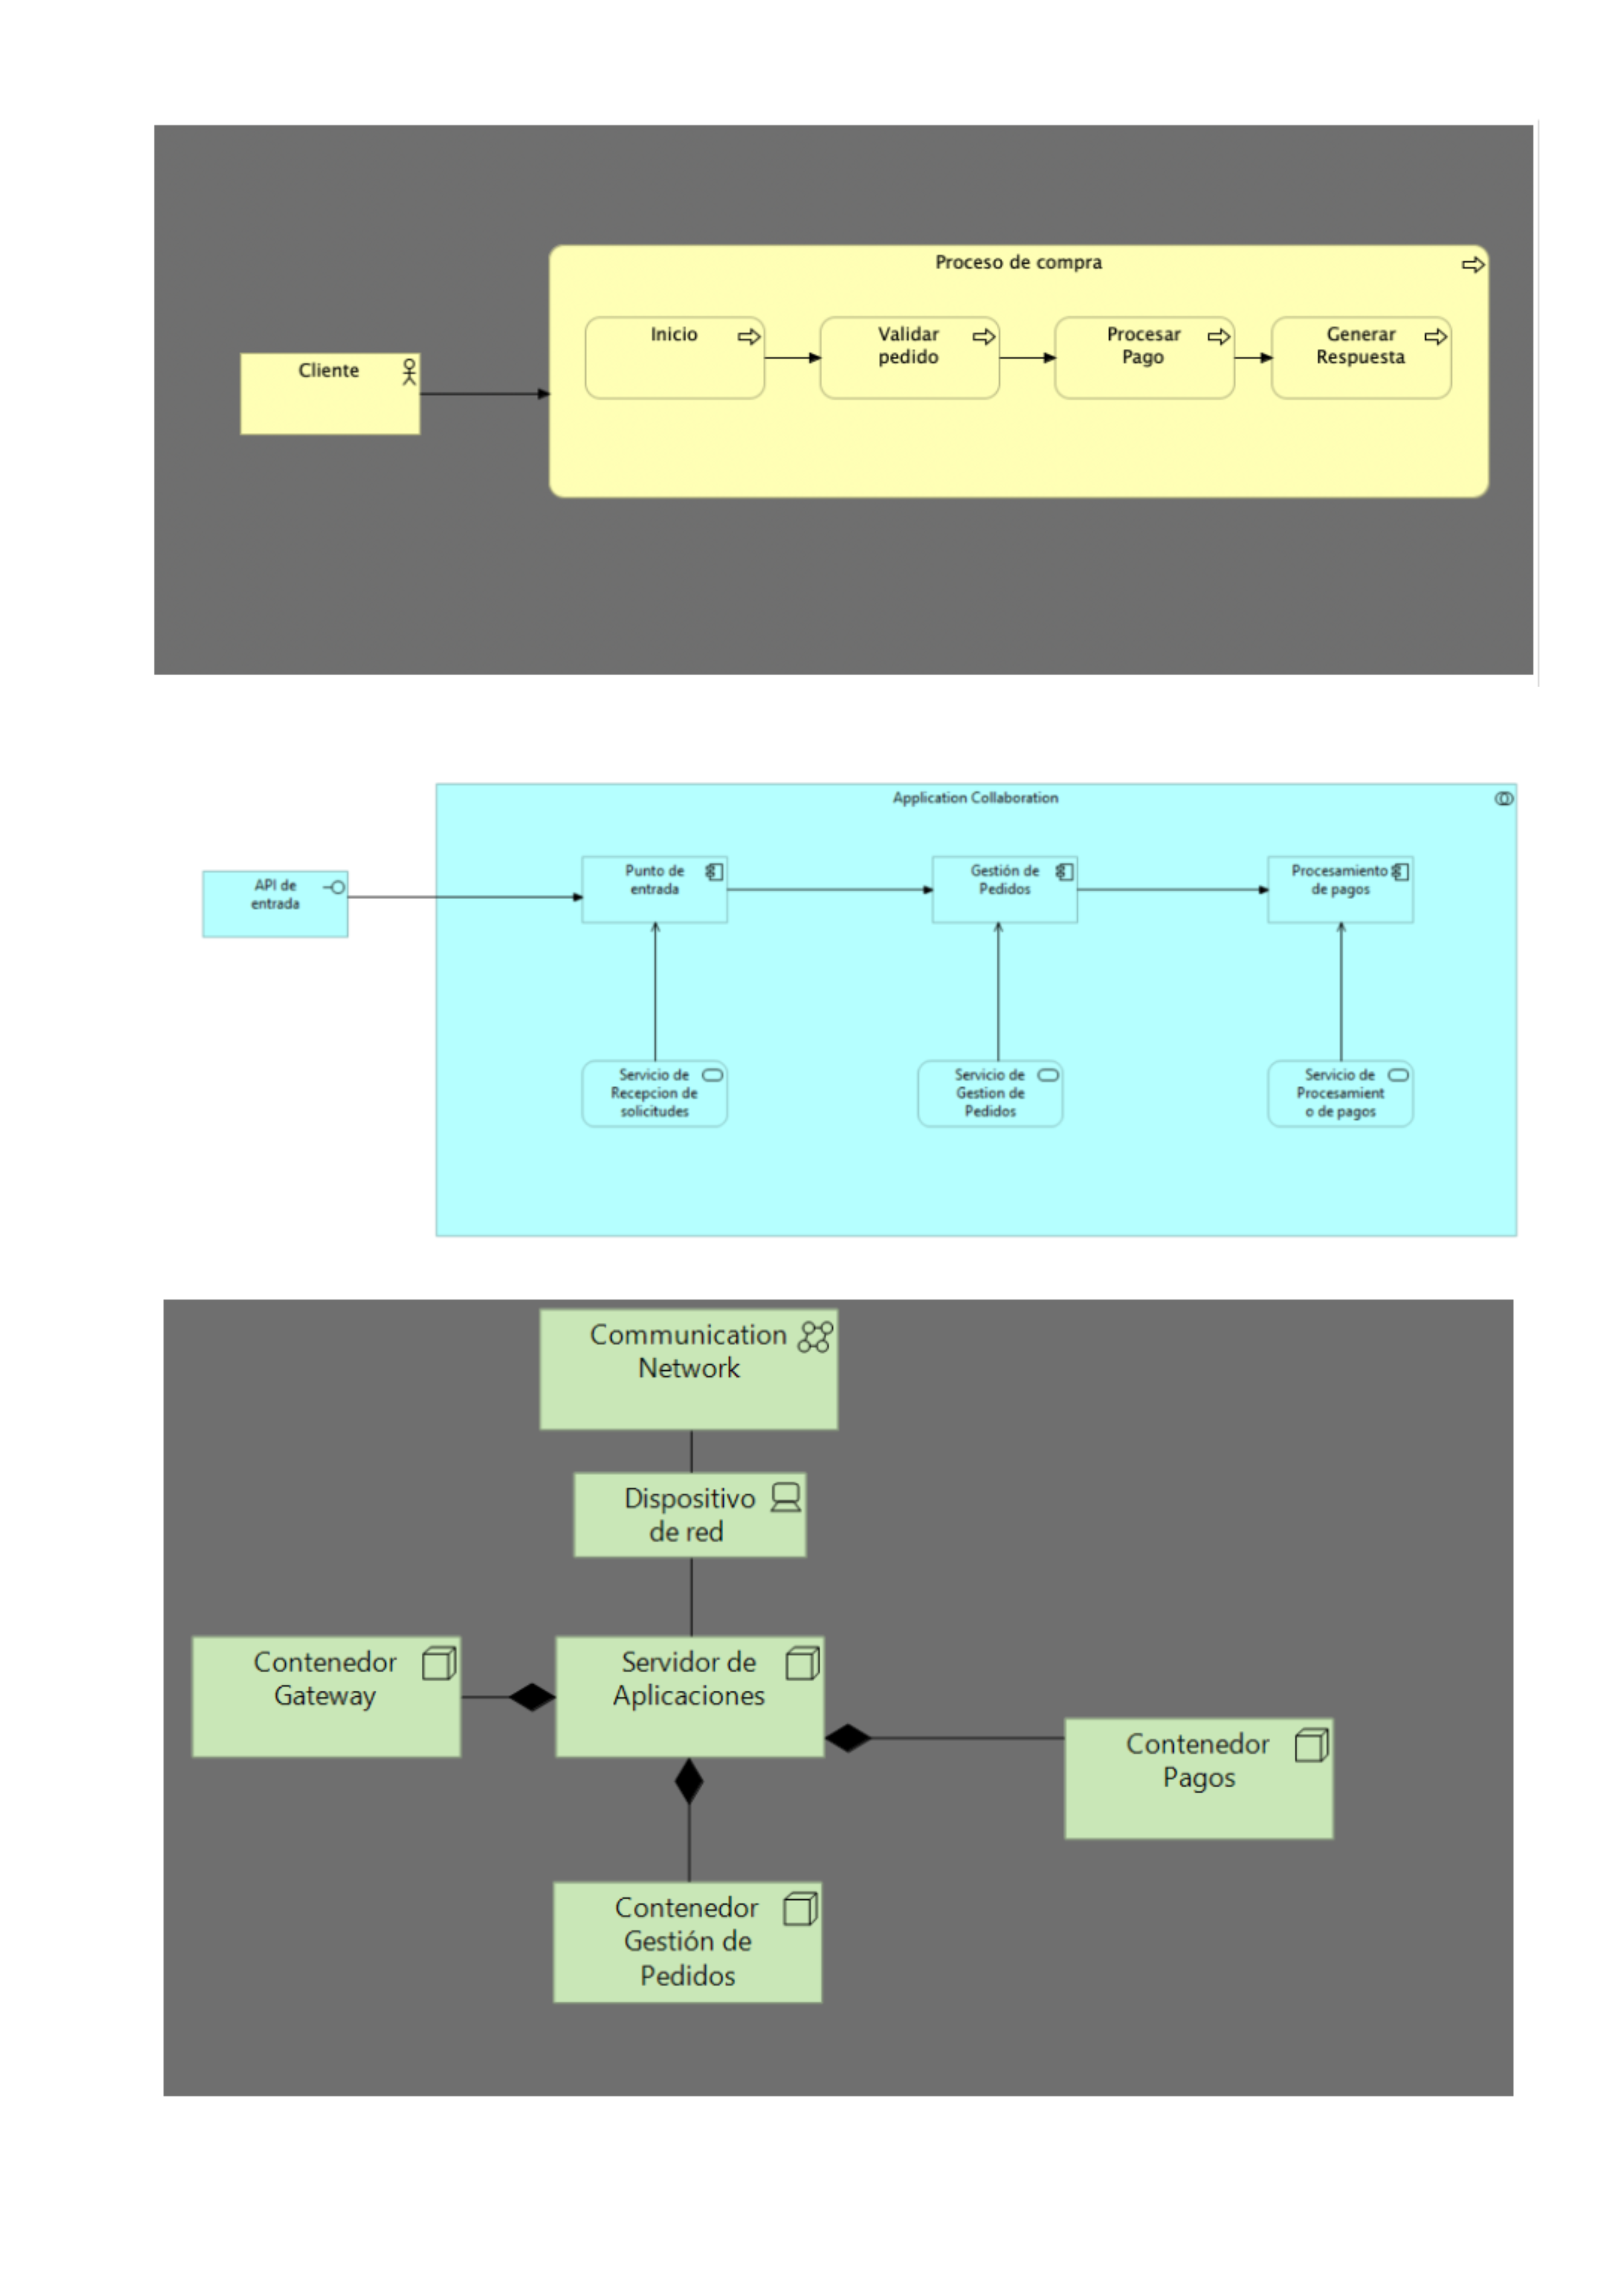
\includegraphics[width=\linewidth,
        height=0.9\textheight,
        keepaspectratio]{tablas-images/diagramas/evaluacion/9S.png}
\caption{Diagrama elaborado por el subgrupo Libre-4}
\label{fig:diagrama_libre4}
\end{figure}

\clearpage
\begin{figure}[H]
\centering
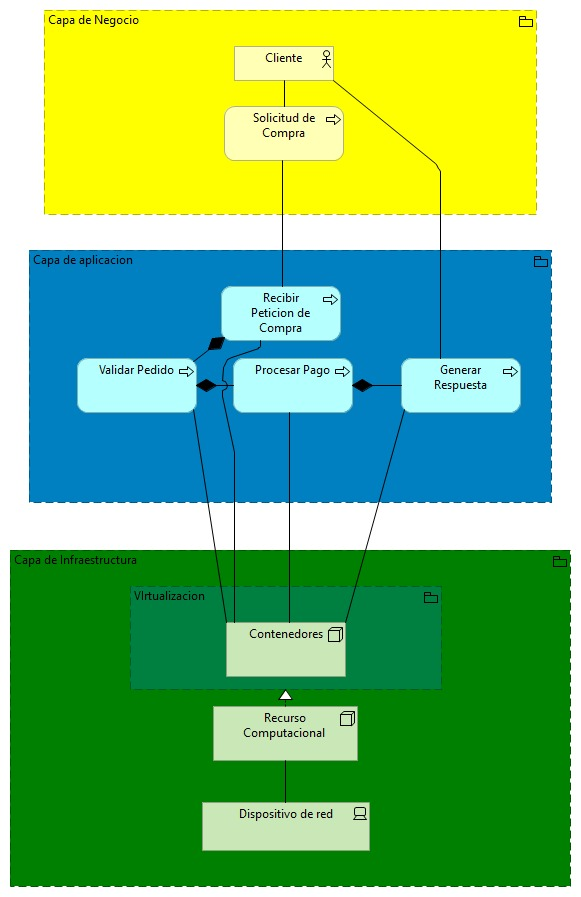
\includegraphics[width=\linewidth,
        height=0.9\textheight,
        keepaspectratio]{tablas-images/diagramas/evaluacion/10S.jpeg}
\caption{Diagrama elaborado por el subgrupo Libre-5}
\label{fig:diagrama_libre5}
\end{figure}

%--------------------------------------------------------------------------------
\FloatBarrier
\cleardoublepage
\refstepcounter{anexo}
\phantomsection
\addcontentsline{toc}{chapter}{Anexo \theanexo: Registro fotográfico del ejercicio de diagramación}

\vspace{40pt}
{\centering \normalfont\huge\bfseries Anexo \theanexo: Registro fotográfico del ejercicio de diagramación \par}
\vspace{40pt}

\label{anx:registro_fotografico}
\markboth{Anexo \theanexo: Registro fotográfico del ejercicio de diagramación}{Anexo \theanexo: Registro fotográfico del ejercicio de diagramación}
\noindent
Las siguientes fotografías corresponden al registro del ejercicio de diagramación realizado con los participantes del estudio. Su publicación cuenta con el consentimiento informado de las personas fotografiadas.
\vfill

\textit{Las imagenes se presentan en las páginas siguientes.}

\begin{figure}[p]
\centering
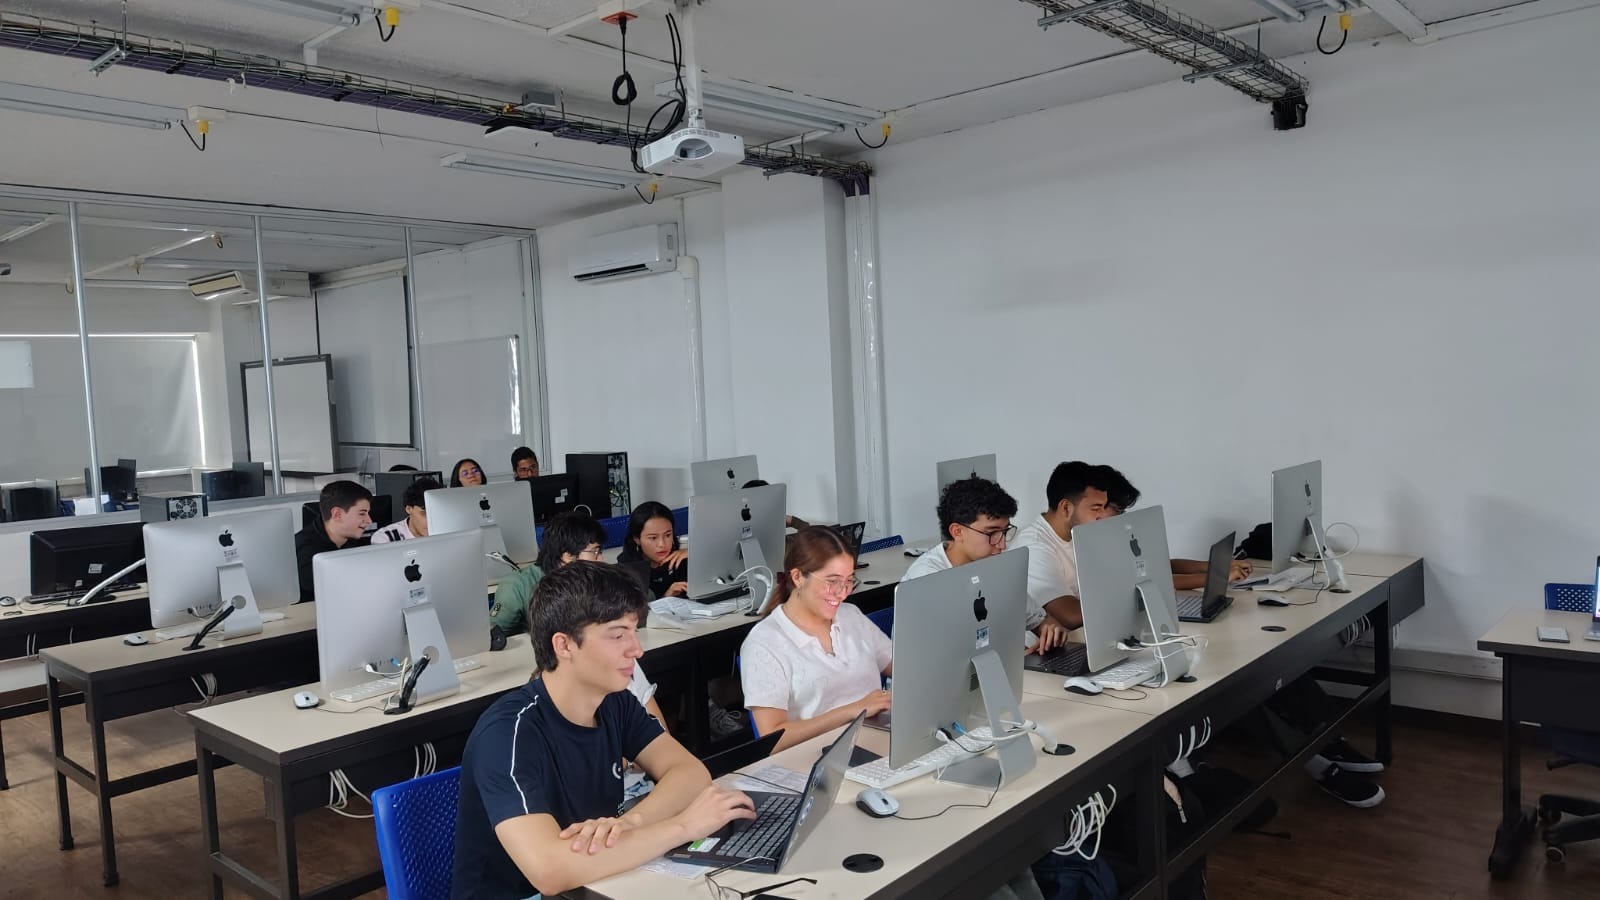
\includegraphics[width=\linewidth,
        height=0.9\textheight,
        keepaspectratio]{tablas-images/fotos/1.jpeg}
\caption{Registro fotográfico del ejercicio de diagramación -- Foto 1}
\label{fig:foto1}
\end{figure}

\clearpage
\begin{figure}[p]
\centering
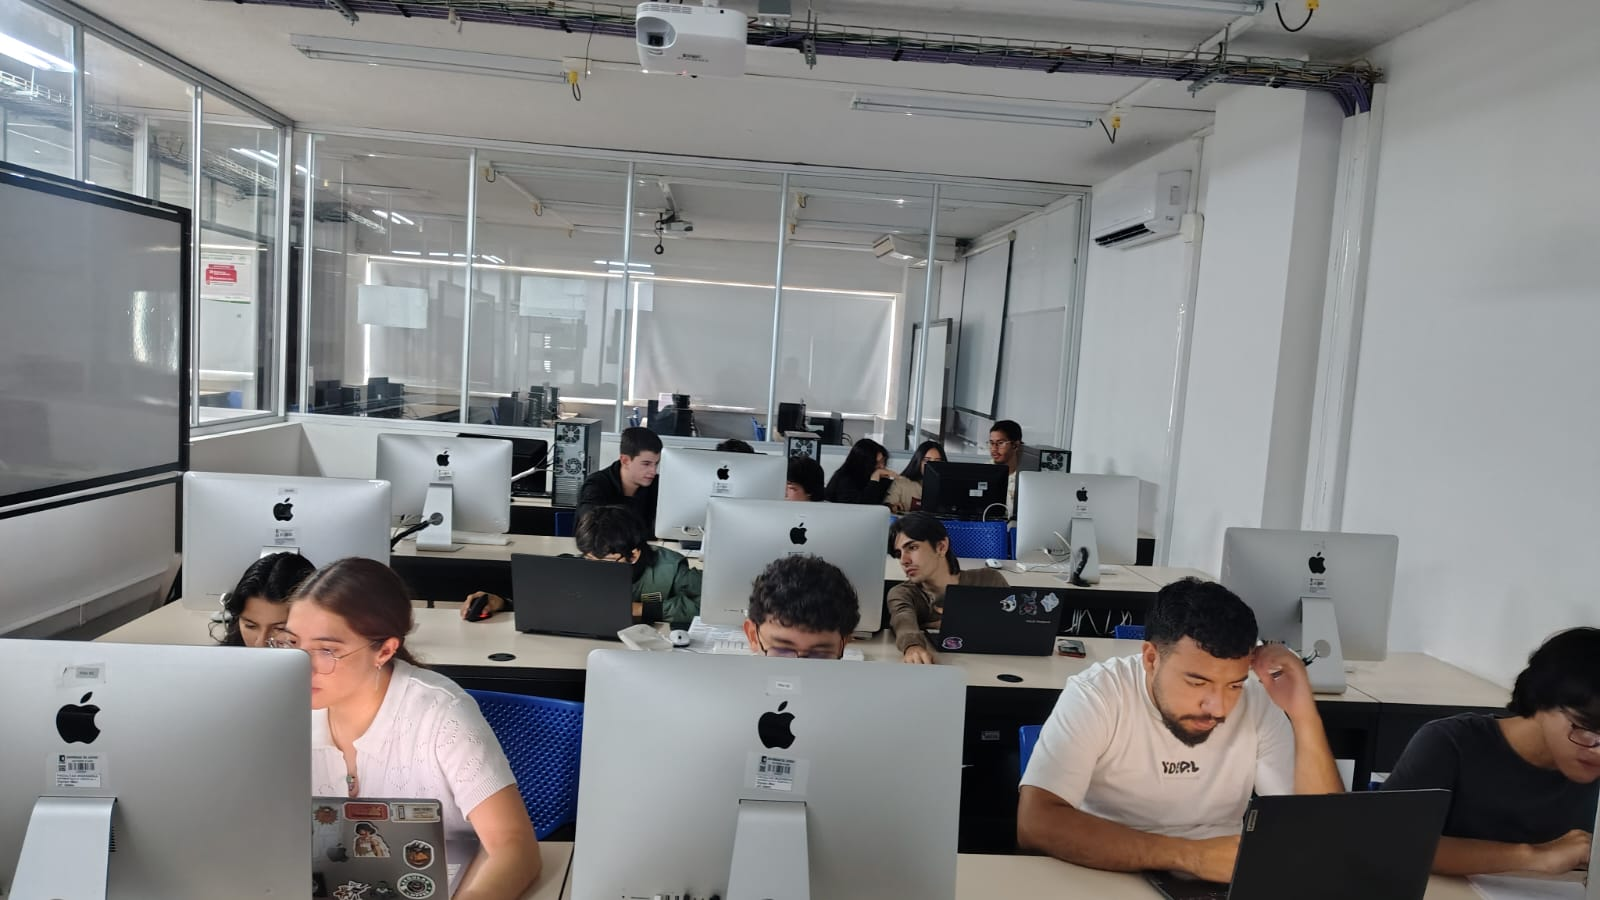
\includegraphics[width=\linewidth,
        height=0.9\textheight,
        keepaspectratio]{tablas-images/fotos/2.jpeg}
\caption{Registro fotográfico del ejercicio de diagramación -- Foto 2}
\label{fig:foto2}
\end{figure}

\clearpage
\begin{figure}[p]
\centering
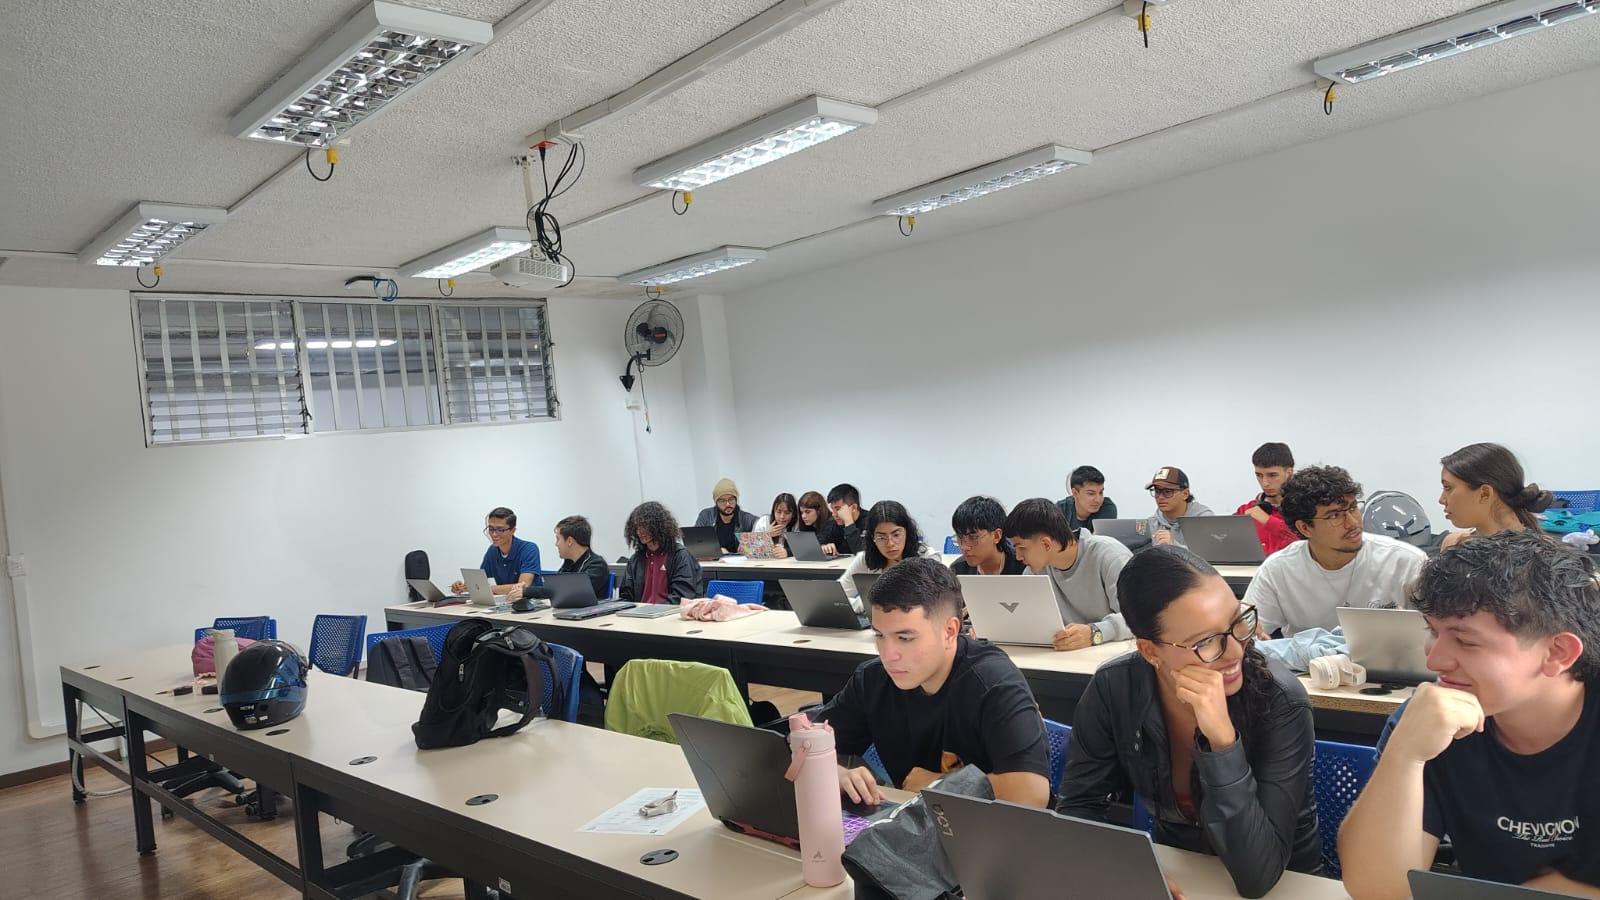
\includegraphics[width=\linewidth,
        height=0.9\textheight,
        keepaspectratio]{tablas-images/fotos/3.jpeg}
\caption{Registro fotográfico del ejercicio de diagramación -- Foto 3}
\label{fig:foto3}
\end{figure}

\clearpage
\begin{figure}[p]
\centering
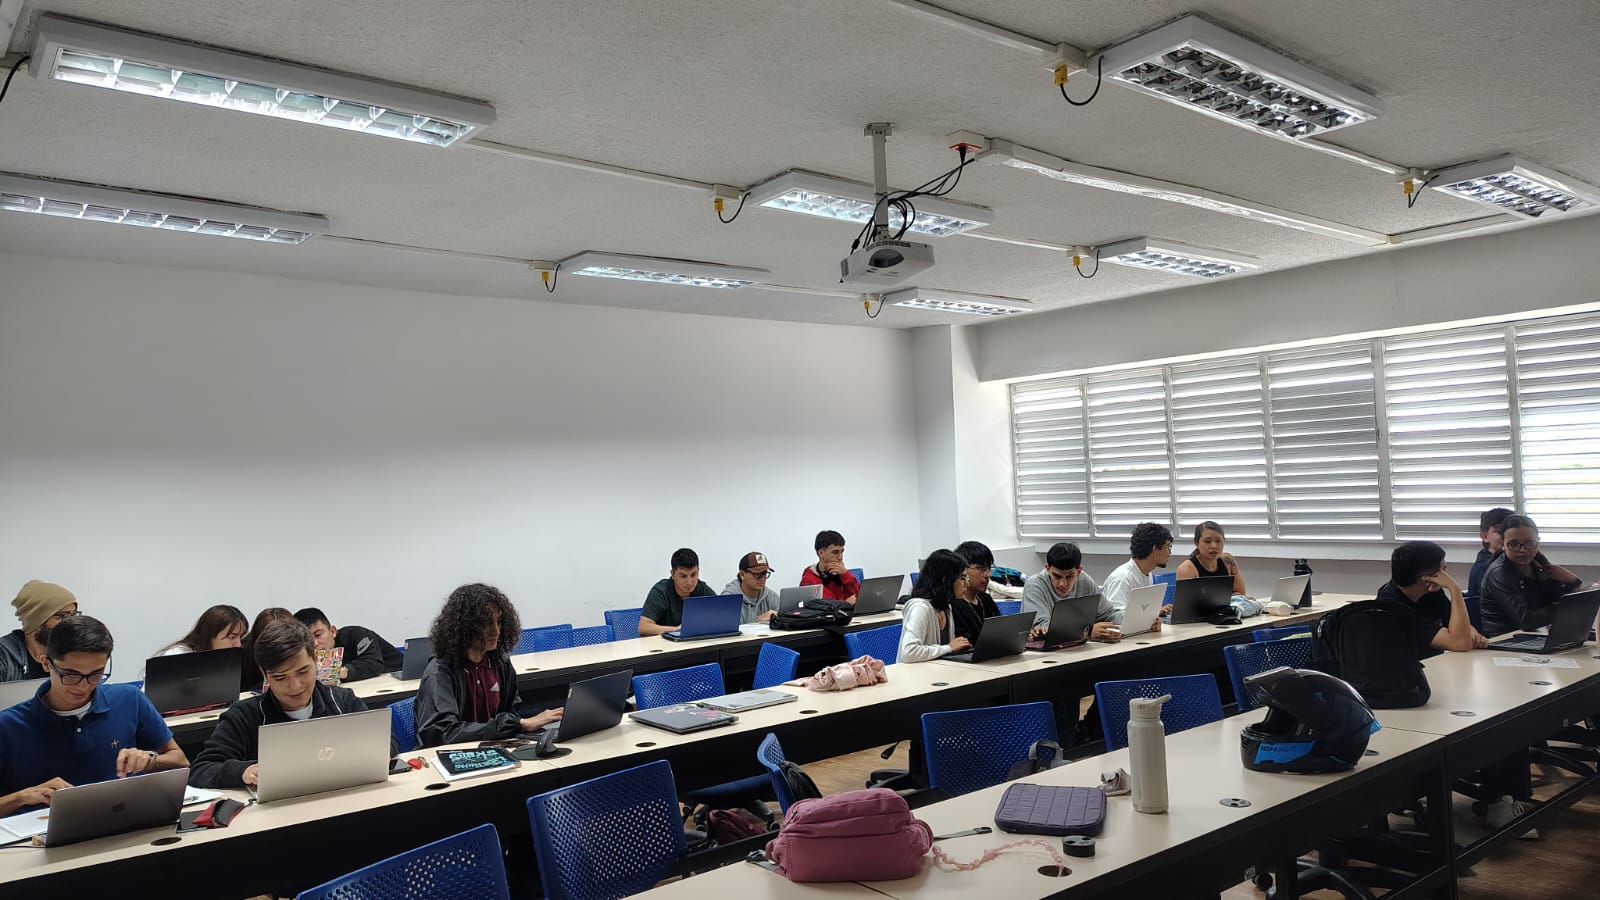
\includegraphics[width=\linewidth,
        height=0.9\textheight,
        keepaspectratio]{tablas-images/fotos/4.jpeg}
\caption{Registro fotográfico del ejercicio de diagramación -- Foto 4}
\label{fig:foto4}
\end{figure}

\clearpage
\begin{figure}[p]
\centering
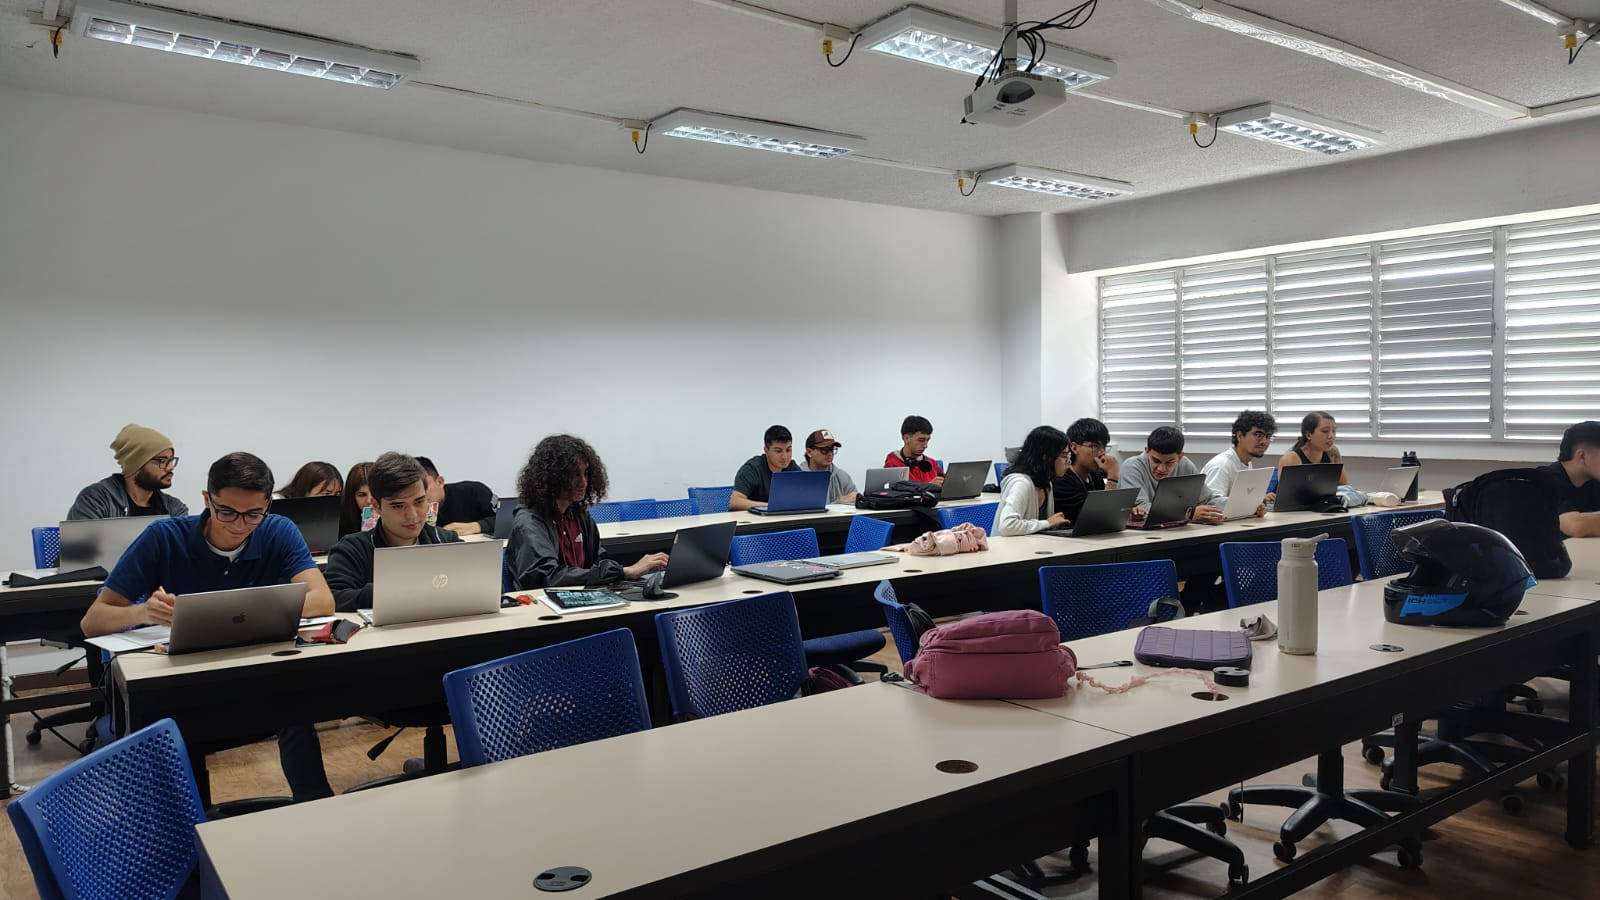
\includegraphics[width=\linewidth,
        height=0.9\textheight,
        keepaspectratio]{tablas-images/fotos/5.jpeg}
\caption{Registro fotográfico del ejercicio de diagramación -- Foto 5}
\label{fig:foto5}
\end{figure}

%--------------------------------------------------------------------------------
\FloatBarrier
% Aquí se pueden agregar más anexos siguiendo el mismo patrón
% \chapter{Título del Anexo B}\label{anexo:nombre-anexo-b}
% \input{ruta/al/archivo.tex}

